% % $RCSfile: proj_proposal.tex,v $
% % $Revision: 1.3 $
% % $Date: 2016/06/10 03:44:08 $
% % $Author: kevin $

\documentclass[11pt, a4paper, twoside, openright]{report}

\usepackage{float} % lets you have non-floating floats
\usepackage{url} % for typesetting urls
\usepackage{graphicx}
\usepackage{subcaption}
\usepackage{hyperref}

\renewcommand{\thesection}{\arabic{section}}

%  We don't want figures to float so we define
%
\newfloat{fig}{thp}{lof}[chapter]
\floatname{fig}{Figure}

% % These are standard LaTeX definitions for the document
% %
\title{Instrumentation System for Liquid Drop Impact and Evaporation}
\author{Daniel Eisen}

% % This file can be used for creating a wide range of reports
% %  across various Schools
% %
% % Set up some things, mostly for the front page, for your specific document
%
% Current options are:
% [ecs|msor|sms]          Which school you are in.
%                         (msor option retained for reproducing old data)
% [bschonscomp|mcompsci]  Which degree you are doing
%                          You can also specify any other degree by name
%                          (see below)
% [font|image]            Use a font or an image for the VUW logo
%                          The font option will only work on ECS systems
%
\usepackage[image,ecs]{vuwproject} 

% You should specifiy your supervisor here with
\supervisor{Gideon Gouws}
% use \supervisors if there are more than one supervisor
\otherdegree{Bachelor of Engineering with Honours}
% Unless you've used the bschonscomp or mcompsci
%  options above use
%   \otherdegree{OTHER DEGREE OR DIPLOMA NAME}
% here to specify degree

% Comment this out if you want the date printed.
\date{}

\begin{document}

% Make the page numbering roman, until after the contents, etc.
\frontmatter

% %% %% %% %% %% %% %% %% %% %% %% %% %% %% %% %% %% %% %% %% %% %% %% %% %% %% %%

\begin{abstract}
\end{abstract}

% %% %% %% %% %% %% %% %% %% %% %% %% %% %% %% %% %% %% %% %% %% %% %% %% %% %% %%

\maketitle
\tableofcontents

% we want a list of the figures we defined
%\listof{fig}{Figures}

% %% %% %% %% %% %% %% %% %% %% %% %% %% %% %% %% %% %% %% %% %% %% %% %% %% %% %%

\mainmatter

% %% %% %% %% %% %% %% %% %% %% %% %% %% %% %% %% %% %% %% %% %% %% %% %% %% %% %%

\section{Introduction}
\textit{Will be an executive summery of following sections, mention who's research this fits into, requirement for budget to cover manufacturing cost etc, and that Will will be a contributor to an auxiliary project that affects this.}

\section{The Problem}
This project is concerned with the development of a instrumentation rig for the study of droplet impact and drying. It is primarily/initially motivated by the powdered milk production process, specifically the behaviour of the drying and collision of concentrated milk droplets. Furthermore, the research, and developed method and procedure can be applicable to various industries. \\

To effectively investigate the behaviour, a variety of aspects can be tracked and characterised during a microscale equivalent lab process, from differing temperatures, substrates, volume, and concentrations. \\

Currently there is an existing platform for the dispensing of droplets and data capture using high speed cameras and other various sensors. It has limitations due to manual control of starting the cameras capture and temperature capturing as well as requiring the operator to position and dispense the droplet by hand. \\

This project will therefore, focus on the design and evaluation of the third generation of this platform with the aim to design and integrate various new subsystems and evaluate their performance against the criteria of improving the reliability and repeatability of the experiments as much as possible.

\subsection{Background and Applications}
...

\section{Proposed Solution}

Evaluate current systems results and identify its short comings. Produce evaluation data and bibliography (est. x wks)
\begin{itemize}
  \item Repeatability of dispensed droplet parameters (position, volume (size), contact angle) and correlate and/or see how the variation in these parameters effects the observed temperature profile and physical behaviours of the droplet throughout the evaporation process.
  \item Identify other sources of variation, such as humidity etc and their weight of influence (whether perusing a solution is worthwhile)
  \item Compare with similar solutions in literature to gain more insight into required design consideration and constraints.
\end{itemize}



\subsection{Base Deliverables}
\begin{itemize}
  \item Mechanical designs to hold, centre, and clamp the substrate stack (fig \ref{fig::old_rig}) together.
  \item Eva
  \item (Main) Improve stability of droplet release stage - possibly electronic pipette, motorized stage etc
\end{itemize}

\subsection{Stretch Goals}
\begin{itemize}
  \item Synchronous data collection, i.e. cameras, temperature, droplet
  \item Atmospheric control enclosure
  \item \dots
\end{itemize}

\begin{figure}
  \begin{subfigure}{.5\textwidth}
    \centering
    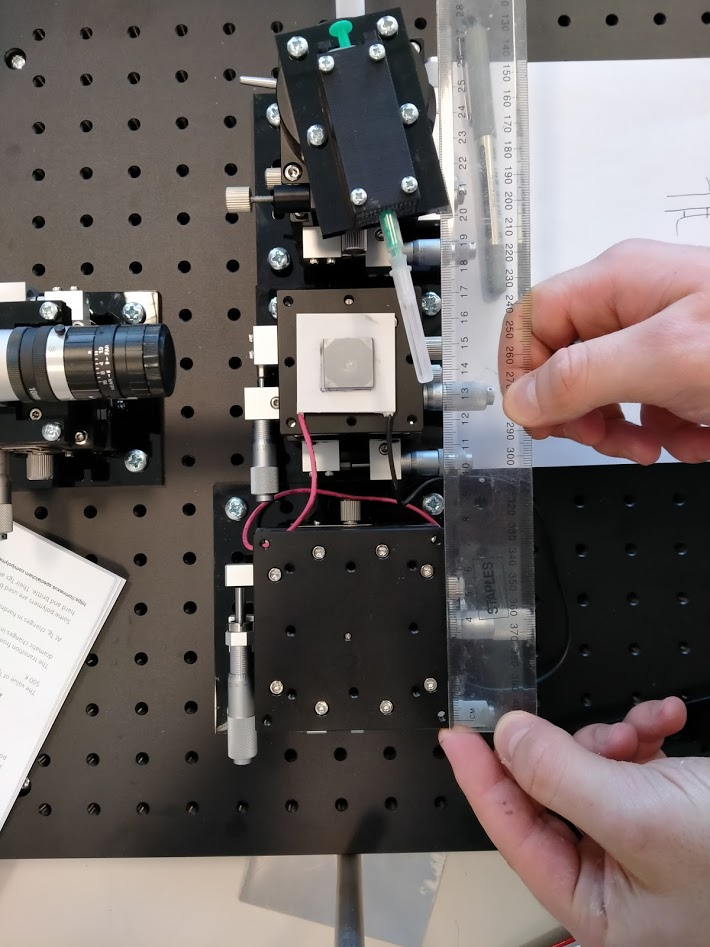
\includegraphics[height=.75\linewidth]{Figures/Full_rig_top.jpg}
    \caption{Full Top View}
  \end{subfigure}%
  \begin{subfigure}{.5\textwidth}
    \centering
    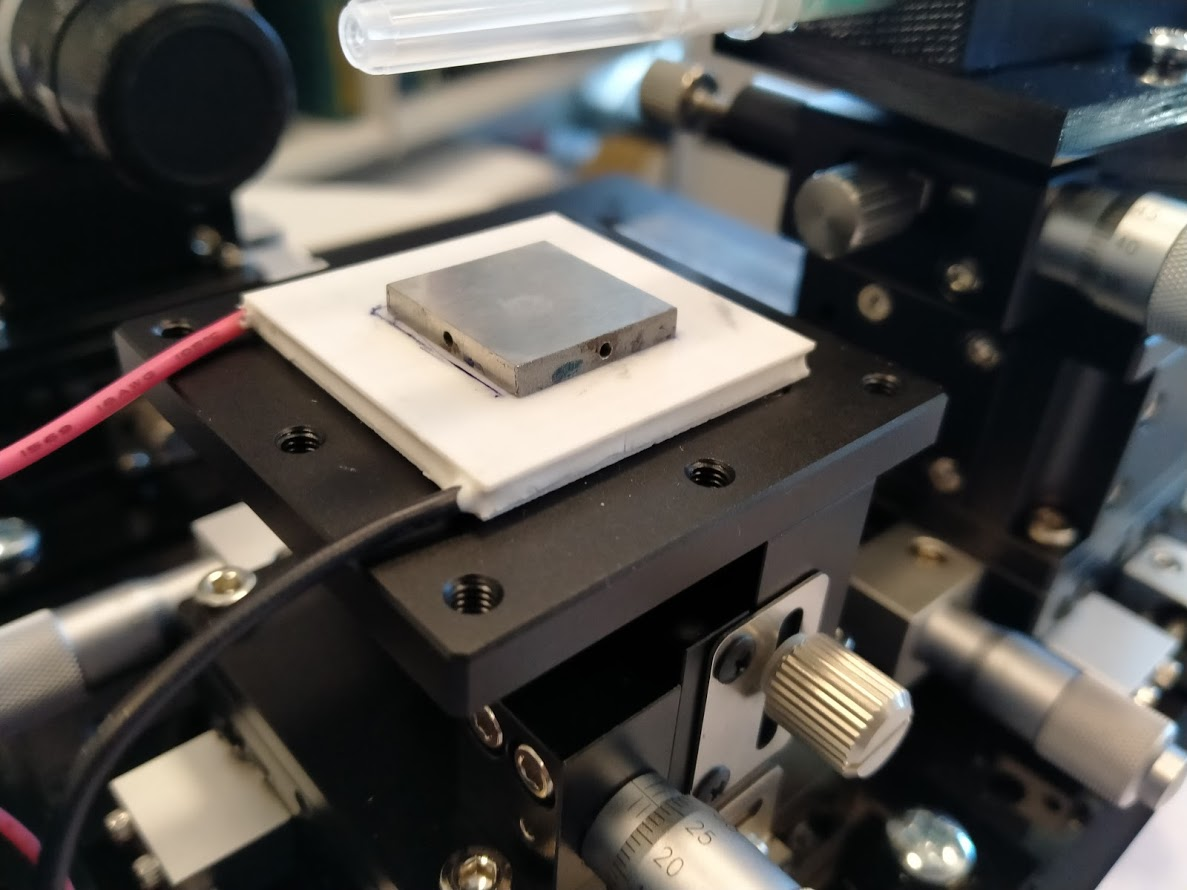
\includegraphics[height=.75\linewidth]{Figures/substrate_stack.jpg}
    \caption{Substrate Stack close-up}
  \end{subfigure}
  \caption{Previous Rig Assembly (bar top camera)}
  \label{fig::old_rig}
  \end{figure}

\newpage
\subsection{Timeline}
\begin{figure}[h]
  \centering
  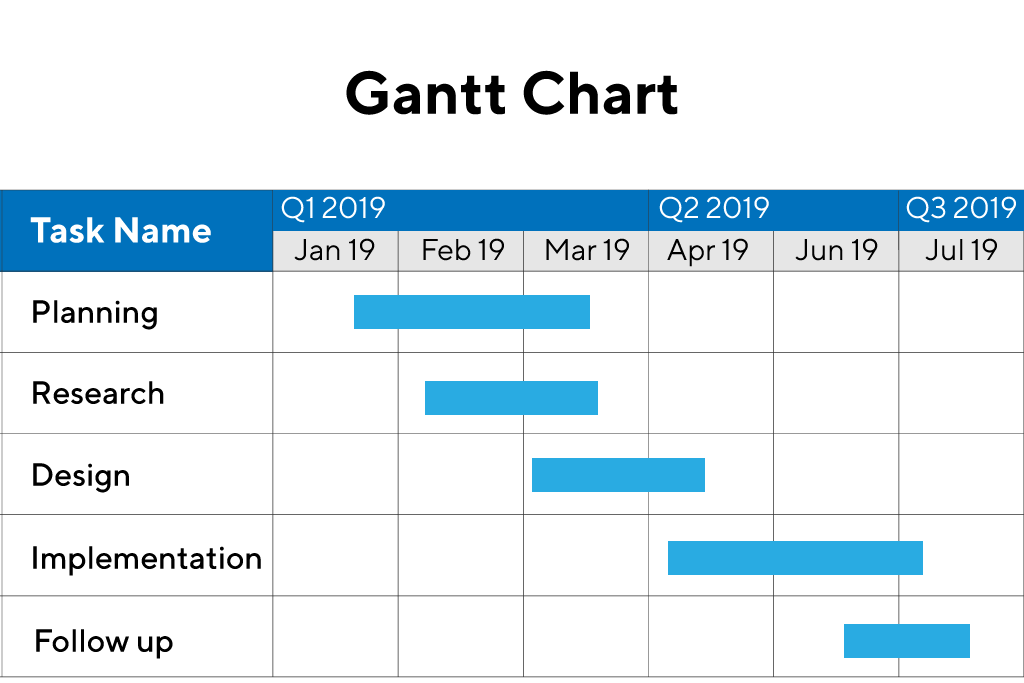
\includegraphics[width=0.5\textwidth]{Figures/Gantt-chart_filler.png}
  \caption{Example Gantt Chart filler, will be replaced with actual timeline}
\end{figure}

\section{Evaluating your Solution}
The work done will be evaluated based on the comparative performance of the development subsystems to improve reliability and repeatability of experimental data and how the work provides a significant contribution the process. 

\section{Resource Requirements}

\subsection{Facilities and Tools}
\begin{itemize}
  \item Labs AM219 and LB207
  \item Computer with SolidWorks, LabView, and other data processing tools
  \item Electronics Test bench (PSU, signal generator, scope etc)
  \item Access to fabrication workshop
\end{itemize}

\subsection{Health and Safety}
\begin{itemize}
  \item Lab Introduction
  \item Peltier Heaters
  \item Basic electric concerns etc
\end{itemize}


\subsection{Budget}
It is worth noting that the instrumentation platform is largely constructed with all its major components, and most needed parts for the design and development of the project are already present.

Given this, the project has estimated a budgetary restriction of \$400.
\begin{itemize}
  \item \$200 to cover workshop manufacturing costs of mechanical designs
  \item \$200 for the purchase stepper motors and auxiliary components, PCB design and manufacture and all other electronic component costing. 
\end{itemize}

\section{COVID-19 Alert Level Management}
Level and planned work that can be achieved and undertaken at the various levels.
\subsection{Level 1}
\subsection{Level 2}
\subsection{Level 3}
\subsection{Level 4}


% %% %% %% %% %% %% %% %% %% %% %% %% %% %% %% %% %% %% %% %% %% %% %% %% %% %% %%
\backmatter
% %% %% %% %% %% %% %% %% %% %% %% %% %% %% %% %% %% %% %% %% %% %% %% %% %% %% %%

\nocite{*}
\bibliographystyle{ieeetr}
\bibliography{sample}
\end{document}
